\documentclass[a4paper,11pt]{article}
\usepackage[utf8]{inputenc}
\usepackage{amsfonts}
\usepackage{graphicx}
%opening
\title{A spatial Poisson transmission model for Ebola (and other diseases)}
\author{Thibaut, Pierre, Anne, Nick G. and the Ebola team}

\begin{document}

\maketitle

\begin{center}
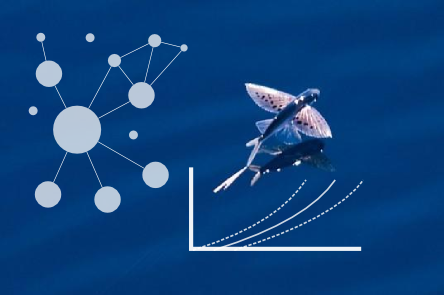
\includegraphics{figs/spatialPoisson} 
\end{center}

\begin{abstract}
The model is a meta-population model using a known (spatial) connectivity matrix between patches and a simple kernel to model dispersal. 
The model is based on incidence data, with only infected individuals being 
known.
Optionally, it can include infection from an unsampled reservoir.
Unlike \textit{outbreaker}, we are not trying to model individual ancestries, 
but merely dynamics within and between patches.
In its simplest form, the model has only two parameters and its likelihood can 
be computed very fast.
More complex extensions can allow for time-varying reproduction number, and/or 
time/spatially varying infection from the reservoir.
\end{abstract}

\newpage
%%%%%%%%%%%%%%%%%%%%%%%
%%%%%%%%%%%%%%%%%%%%%%%
\section{Notations}
%%%%%%%%%%%%%%%%%%%%%%%
%%%%%%%%%%%%%%%%%%%%%%%

\begin{itemize}
 \item $T$: number of time steps in the data
 \item $P$: number of patches
 \item $I_t^i$: observed incidence in patch $i$ at time $t$ (data)
 \item $N_t^i$: true, unobserved incidence in patch $i$ at time $t$ (augmented 
data)
 \item $I_t, N_t$: vectors of (observed, true) incidence of all patches 
 ($I_t = (I_t^1, \ldots, I_t^P)$; $N_t = (N_t^1, \ldots, N_t^P)$)
 \item $I,N$: matrix of observed / true incidence of all patches at all time 
steps ($I = (I_1, \ldots, I_T)$; $N = (N_1, \ldots, N_T)$
 \item $I_{1 \rightarrow t}, N_{1 \rightarrow t}$: matrices of observed / true 
incidence from time 1 to time $t$ 
($I_{1 \rightarrow t} = (I_1, \ldots, I_t)$; $N_{1 \rightarrow t} = (N_1, 
\ldots, N_t)$
 \item $D_{ij}$: distance between $i$ and $j$
 \item $w(.)$: the known probability mass distribution of the generation time / serial interval
%  \item $n_t^i$: the number of infected individuals in patch $i$ at time $t$
 \item $d_{j\rightarrow i}$: intensity of dispersion from $j$ to $i$
 \item $\delta$: general dispersal parameter
%  \item $\phi$: background force of infection
 \item $\pi$: proportion of cases reported
 \item $\rho$: estimated (hyper)parameters of the distribution of $R$
 \item $R$: the effective reproduction 
number
%  \item $t_k$: the date of infection of individual $k$
%  \item $f_\mathcal{P}(a,b)$: the Poisson density for $a$ observations and a rate $b$
 \item $k(a,b)$: a spatial kernel for a distance $a$ and a parameter $b$
 \item $\theta_{\delta}$: (fixed) parameter for the prior of 
$\delta$
 \item $\theta_{\pi}$: (fixed) parameter for the prior of $\pi$
\end{itemize}





%%%%%%%%%%%%%%%%%%%%%%%
%%%%%%%%%%%%%%%%%%%%%%%
\section{Model}
%%%%%%%%%%%%%%%%%%%%%%%
%%%%%%%%%%%%%%%%%%%%%%%

We want to sample from the posterior distribution proportional to:
\begin{equation}
 p(I, N, R, \rho, \delta, \pi) = p(I, N | R, \rho, \delta, \pi)  
 p(R, \rho, \delta, \pi)
\end{equation}
which can be rewritten
\begin{equation}
\underbrace{p(I | N, \pi) p(N | R, \delta) p(R | \rho) }_{likelihood} 
\underbrace{p(\rho) p(\delta) p(\pi)}_{priors} 
\end{equation}

The term $p(I | N, \pi)$ is the probability of the observed incidence given the 
true incidence $N$ and the reporting probability $\pi$.
It is computed as:
\begin{equation}
p(I | N, \pi) = \prod_{i}\prod_{t} p(I_t^i| N_t^i, \pi)
\end{equation}
with:
\begin{equation}
p(I_t^i| N_t^i, \pi) = f_\mathcal{B}(I_t^i, N_t^i, \pi)
\end{equation}
where $f_\mathcal{B}(x,a,b)$ is the Binomial p.m.f. for $x$ successes, $a$ draws 
and a probability $b$.
\\

The term $p(N | R, \delta)$ is the probability of the true incidence 
given the infectivity in the system and the spatial processes at play.
It is computed as:

\begin{eqnarray}
p(N | R, \delta) & = & p(N_1, \ldots, N_t | R, \delta)\\
 & = & \underbrace{(N_1| R, \delta)}_{constant} p(N_2| N_1, R, \delta) \ldots 
       p(N_t| N_1, \ldots, N_{t-1}, R, \delta) \\
 & \propto & \prod_{t=2}^T p(N_t| N_{1 \rightarrow t-1}, R, \delta)\\
 & = & \prod_{t=2}^T \prod_{i=1}^P 
       p(N_t^i| N_{1 \rightarrow t-1}, R, \delta)\\
\end{eqnarray}
with:
\begin{equation}
p(N_t^i| N_{1 \rightarrow t-1}, R, \delta) = f_\mathcal{P}(N_t^i, \lambda_t^i)
\end{equation}
where $f_\mathcal{P}$ if the p.m.f of a Poisson distribution and $\lambda_t^i$ 
the force of infection towards patch $i$ and time $t$.
$\lambda_t^i$ is a sum over of the forces of infection of all patches towards $i$ (including $i \rightarrow i$). 
We note $\beta_t^j$ the global infectiousness coming from infected individuals 
in patch $j$ at time $t$, defined by the renewal equation:
\begin{equation}
 \beta_t^j = \sum_{s=1}^{t-1} N_s^j \:  w(t - s)
\end{equation}
The force of infection experienced by patch $i$ at time $t$ is then:
\begin{equation}
\lambda_t^i = R \sum_{j=1}^P \beta_t^j \: k(d_{j\rightarrow i},\delta)
\end{equation}
where $R$ is the reproduction number. 
The likelihood of the augmented data is thus given by:
\begin{equation}
p(N|R, \delta) \propto \prod_{t=2}^T \prod_{i=1}^P 
       f_\mathcal{P}(N_t^i, R 
       \sum_{j=1}^P \sum_{s=1}^{t-1} N_s^j \:  w(t - s) \:
       k(d_{j\rightarrow i},\delta) )
\end{equation}


Note that we can easily turn it into a time-dependent term $R_t$, in which 
case 
we will have to assume i) a functional form or ii) $R_t$ constant 
between break-points. 
Similarly, it can be turned into a patch-specific $R_i$, in which case 
heterogeneity between patches can be modeled using a given distribution.
For the time being, heterogeneity in $R$ across space and time will be modelled 
using a gamma distribution:
\begin{equation}
p(R | \rho) = f_{\gamma} (R, \rho_1, \rho_2)
\end{equation}
where $\rho$ is a vector containing the mean $\rho_1$ and variance
$\rho_2$ of a gamma distribution.
The corresponding shape parameter $\alpha$ is:
\begin{equation}
\alpha = \frac{\rho_1^2}{\rho_2}
\end{equation}
and the corresponding rate parameter $\beta$ is:
\begin{equation}
\beta = \frac{\rho_1}{\rho_2}
\end{equation}
\\

The prior of $\rho_1$ and $\rho_2$ are normally distributed; by default we 
use:
\begin{equation}
\rho_1 \sim \mathcal{N}(3,0.5) \mbox{ and } \rho_2 \sim \mathcal{N}(6,0.5)
\end{equation}


The prior of $\delta$ is an exponential distribution of parameter 
$\theta_{\delta}$:
\begin{equation}
p(\delta) = f_{exp}(\delta,  \theta_{\delta})
\end{equation}
The prior of $\pi$ is a beta distribution of parameter 
$\theta_{\pi}$:
\begin{equation}
p(\pi) = f_{beta}(\delta,  \theta_{\pi})
\end{equation}





%%%%%%%%%%%%%%%%%%%%%%%
%%%%%%%%%%%%%%%%%%%%%%%
\section{Data augmentation: Gibbs sampler}
%%%%%%%%%%%%%%%%%%%%%%%
%%%%%%%%%%%%%%%%%%%%%%%

We seek a Gibbs sampler for the augmented incidence at time $t$, $N_t$.
For this, we need to know (up to an additive or multiplicative constant) the 
distribution of $N_t$ conditional on everything else:
\begin{eqnarray}
p(N_t | N_{1 \rightarrow t-1}, I_{1 \rightarrow t-1}, R, \rho, \delta, \pi) 
\propto p(N_{1 \rightarrow t}, I_{1 \rightarrow t}, R, \rho, \delta, \pi) \\
\propto p( I_{1 \rightarrow t} | N_{1 \rightarrow t}, \pi) 
p(N_t | N_{1 \rightarrow t-1},  R, \delta) \\
= (\prod_{s=1}^t p(I_s| N_s, \pi)) \:\:
p(N_t | N_{1 \rightarrow t-1}, R, \delta))  \\
\propto p(I_t | N_t, \pi) \:\:
p(N_t | N_{1 \rightarrow t-1},  R, \delta)\\
= (\prod_{j=1}^P f_{\mathcal{B}}(I_t^j, N_t^j, \pi))
(\prod_{j=1}^P  f_{\mathcal{P}}(N_t^j, \lambda_t^j))\\
= \prod_{j=1}^P [ {N_t^j \choose I_t^j} \pi^{I_t^j} 
(1-\pi)^{N_t^j - I_t^j} \:\: 
\frac{{\lambda_t^j}^{N_t^j} e^{-\lambda_t^j}}{N_t^j!}]\\
\propto \prod_{j=1}^P [ \frac{N_t^j!}{I_t^j!(N_t^j-I_t^j)!} 
(1-\pi)^{N_t^j - I_t^j} \:\: 
\frac{{\lambda_t^j}^{N_t^j}}{N_t^j!}]\\
\propto \prod_{j=1}^P [ \frac{1}{(N_t^j-I_t^j)!} 
(1-\pi)^{N_t^j - I_t^j} \:\: 
{\lambda_t^j}^{N_t^j - I_t^j}{\lambda_t^j}^{I_t^j}]\\
\propto \prod_{j=1}^P \frac{1}{(N_t^j-I_t^j)!} 
[(1-\pi)\lambda_t^j]^{N_t^j - I_t^j}\\
\propto \prod_{j=1}^P f_{\mathcal{P}}(N_t^j-I_t^j , (1-\pi)\lambda_t^j)
\end{eqnarray}
The conditional distribution of $N_t$ is therefore proportional to the 
probability of the number of unobserved cases $N_t^j-I_t^j$, given by a Poisson 
distribution of rate $(1-\pi)\lambda_t^j$. This is an intuitive result: the 
actual incidence is larger for smaller reporting rates ($\pi$) and higher 
forces of infection ($\lambda_t^j$).
In practice, we can derive $N_t$ by sampling directly the number of unobserved 
cases $N_t^j-I_t^j$ from a Poisson distribution of parameter 
$(1-\pi)\lambda_t^j$.

%The likelihood of $I_t$, the incidence vector at time $t$, is defined as:
%\begin{equation}
%p(I_t | R, \delta) = \prod_{i=1}^P f_\mathcal{P}(I_t^i, \lambda_t^i)
%\end{equation}
%where $f_\mathcal{P}$ is the $pmf$ of a Poisson distribution.
%\\
%
%By extension, the likelihood for the entire data is:
%\begin{equation}
%p(I_1, \ldots, I_t | R, \delta) = \prod_{t=1}^T \prod_{i=1}^P 
%f_\mathcal{P}(I_t^i, \lambda_t^i)
%\end{equation}
%


%
%%%%%%%%%%%%%%%%%%%%%%%%
%%%%%%%%%%%%%%%%%%%%%%%%
%\section{Unobserved reservoir}
%%%%%%%%%%%%%%%%%%%%%%%%
%%%%%%%%%%%%%%%%%%%%%%%%
%
%So far the model assumes that all patches are known, and the connectivity 
%between the patches is known as well -- up to a dispersal parameter $\delta$.
%An unobserved reservoir (e.g. zoonotic cases) can be added using a few 
%assumptions. 
%To model the reservoir, we need to estimate the force of infection coming from 
%the reservoir to the different patches:
%\begin{equation}
%\phi_t^i = d_{res \rightarrow i} \beta_t^{res}
%\end{equation}
%
%We can make different assumptions on the two components, depending on whether 
%we are interested in modeling spatial or temporal heterogeneity.
%The simplest approach is to assume a constant 
%force of infection over time and equal across patches, in which case only one 
%additional parameter needs to be estimated.
%A more flexible approach would be to use a distribution of $\phi_t^i$ to 
%account for heterogeneity between patches.
%This is still a parsimonious approach in terms of parameters (typically 1-2 
%would be needed).

%
%
%%%%%%%%%%%%%%%%%%%%%%%%
%%%%%%%%%%%%%%%%%%%%%%%%
%\section{Complexity}
%%%%%%%%%%%%%%%%%%%%%%%%
%%%%%%%%%%%%%%%%%%%%%%%%
%
%In its simplest form, the model has 2 parameters without reservoir 
%($R$,$\delta$), and 3 with 
%reservoir ($R$,$\delta$,$\phi$).
%Likelihood computation will be fast, as we need only compute Poisson densities, 
%and no data augmentation.
%It can become much more complex with time-varying $R$ and time-varying, 
%spatially heterogeneous infection from the reservoir $\phi$.
%There will probably also be issues trying to estimate time-varying $R$ and 
%$\phi$, as the two effects would be largely confounded.
%

\end{document}
